


%_______________
\newpage\subsection*{Exercises} % Continuous distributions

% 1

\eoce{\qt{Cat weights\label{cat_weights}} The histogram shown below represents 
the weights (in kg) of 47 female and 97 male cats. \footfullcite{cats} \\
\begin{minipage}[c]{0.47\textwidth}
\begin{parts}
\item What fraction of these cats weigh less than 2.5 kg?
\item What fraction of these cats weigh between 2.5 and 2.75 kg?
\item What fraction of these cats weigh between 2.75 and 3.5 kg?
\end{parts} \vspace{27mm}
\end{minipage}
\begin{minipage}[c]{0.05\textwidth}
$\:$ 
\end{minipage}
\begin{minipage}[c]{0.48\textwidth}
\begin{center}
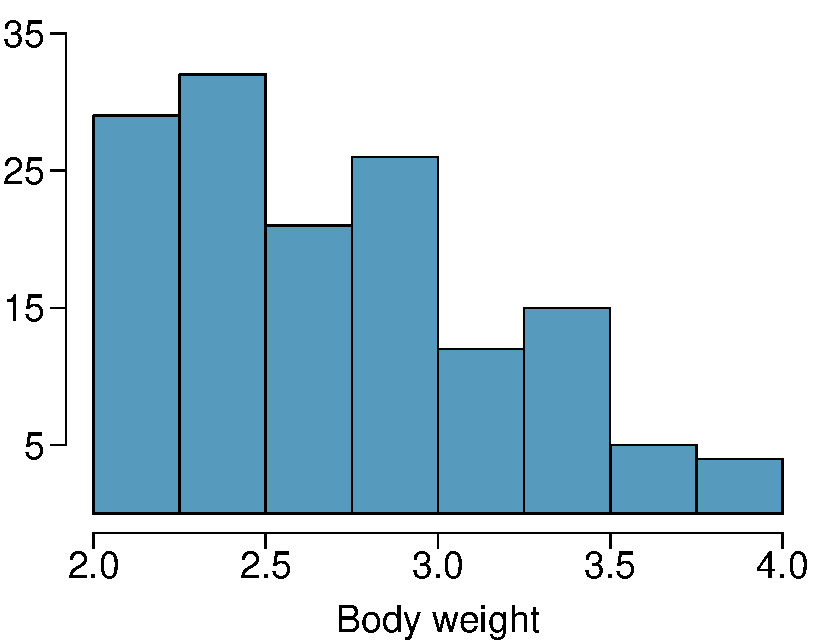
\includegraphics[width=\textwidth]{ch_probability/figures/eoce/cat_weights/cat_weights.pdf}
\end{center}
\end{minipage}
}{}

% 2

\eoce{\qt{Income and gender\label{income_gender}} The relative frequency table 
below displays the distribution of annual total personal income (in 2009 
inflation-adjusted dollars) for a representative sample of 96,420,486 Americans. 
These data come from the American Community Survey for 2005-2009. This sample is 
comprised of 59\% males and 41\% females. \footfullcite{acsIncome2005-2009} \\

\noindent\begin{minipage}[c]{0.60\textwidth}
\begin{parts}
\item Describe the distribution of total personal income.
\item What is the probability that a randomly chosen US resident makes less than 
\$50,000 per year?
\item What is the probability that a randomly chosen US resident makes less than 
\$50,000 per year and is female? Note any assumptions you make.
\item The same data source indicates that 71.8\% of females make less than 
\$50,000 per year. Use this value to determine whether or not the assumption you 
made in part (c) is valid.
\end{parts} 
\end{minipage}
\begin{minipage}[c]{0.4\textwidth}
{\small
\begin{center}
\begin{tabular}{lr}
  \hline
\textit{Income}         & \textit{Total} \\
  \hline
\$1 to \$9,999 or loss  & 2.2\% \\
\$10,000 to \$14,999    & 4.7\% \\
\$15,000 to \$24,999    & 15.8\% \\
\$25,000 to \$34,999    & 18.3\% \\
\$35,000 to \$49,999    & 21.2\% \\
\$50,000 to \$64,999    & 13.9\% \\
\$65,000 to \$74,999    & 5.8\% \\
\$75,000 to \$99,999    & 8.4\% \\
\$100,000 or more       & 9.7\% \\
   \hline
\end{tabular}
\end{center}
}
\end{minipage}
}{}

% 3

\eoce{\qt{Grade distributions\label{grade_dists}} Each row in the table below is 
a proposed grade distribution for a class. Identify each as a valid or invalid 
probability distribution, and explain your reasoning.
\begin{center}
\begin{tabular}{l  ccccc} 
    & \multicolumn{5}{c}{\textit{Grades}} \\
\cline{2-6}
    & A     & B     & C     & D     & F  \\
\cline{2-6}
(a) & 0.3   & 0.3   & 0.3   & 0.2   & 0.1\\
(b) & 0     & 0     & 1     & 0     & 0 \\
(c) & 0.3   & 0.3   & 0.3   & 0     & 0 \\
(d) & 0.3   & 0.5   & 0.2   & 0.1   & -0.1 \\
(e) & 0.2   & 0.4   & 0.2   & 0.1   & 0.1 \\
(f) & 0     & -0.1  & 1.1   & 0     & 0 \\
\end{tabular}
\end{center}
}{}

% 4

\eoce{\qt{Health coverage, frequencies\label{health_coverage_freqs}} The 
Behavioral Risk Factor Surveillance System (BRFSS) is an annual telephone survey 
designed to identify risk factors in the adult population and report emerging 
health trends. The following table summarizes two variables for the respondents: 
health status and health coverage, which describes whether each respondent had 
health insurance. \footfullcite{data:BRFSS2010}
\begin{center}
\begin{tabular}{rrrrrrrr}
                    &       & \multicolumn{5}{c}{\textit{Health Status}} &  \\ 
\cline{3-7}
                    &       & Excellent & Very good & Good  & Fair  & Poor  & Total\\ 
\cline{2-8}
\textit{Health}     & No    & 459       & 727       & 854   & 385   & 99    & 2,524 \\ 
\textit{Coverage}   & Yes   & 4,198     & 6,245     & 4,821 & 1,634 & 578   & 17,476 \\ 
\cline{2-8}
                    & Total & 4,657     & 6,972     & 5,675 & 2,019 & 677   & 20,000
\end{tabular}
\end{center}
\begin{parts}
\item If we draw one individual at random, what is the probability that the 
respondent has excellent health and doesn't have health coverage?
\item If we draw one individual at random, what is the probability that the 
respondent has excellent health or doesn't have health coverage?
\end{parts}
}{}

% 5

\eoce{\qt{HIV in Swaziland\label{tree_hiv_swaziland}} Swaziland has the highest 
HIV prevalence in the world: 25.9\% of this country's population is infected with 
HIV.\footfullcite{ciaFactBookHIV:2012} The ELISA test is one of the first and 
most accurate tests for HIV. For those who carry HIV, the ELISA test is 99.7\% 
accurate. For those who do not carry HIV, the test is 92.6\% accurate. If an 
individual from Swaziland has tested positive, what is the probability that he 
carries HIV?
}{}

% 6

\eoce{\qt{Twins\label{tree_twins}} About 30\% of human twins are identical, and 
the rest are fraternal. Identical twins are necessarily the same sex -- half are 
males and the other half are females. One-quarter of fraternal twins are both 
male, one-quarter both female, and one-half are mixes: one male, one female. You 
have just become a parent of twins and are told they are both girls. Given this 
information, what is the probability that they are identical?
}{}

% 7

\eoce{\qt{Cost of breakfast\label{cost_of_breakfast}} Sally gets a cup of coffee 
and a muffin every day for breakfast from one of the many coffee shops in her 
neighborhood. She picks a coffee shop each morning at random and independently of 
previous days. The average price of a cup of coffee is \$1.40 with a standard 
deviation of 30\textcent (\$0.30), the average price of a muffin is \$2.50 with a 
standard deviation of 15\textcent, and the two prices are independent of each 
other.
\begin{parts}
\item What is the mean and standard deviation of the amount she spends on 
breakfast daily?
\item What is the mean and standard deviation of the amount she spends on 
breakfast weekly (7~days)?
\end{parts}
}{}

% 8

\eoce{\qt{Scooping ice cream\label{scoop_ice_cream}} Ice cream usually comes in 1.5 
quart boxes (48 fluid ounces), and ice cream scoops hold about 2 ounces. 
However, there is some variability in the amount of ice cream in a box as well as 
the amount of ice cream scooped out. We represent the amount of ice cream in the 
box as $X$ and the amount scooped out as $Y$. Suppose these random variables have 
the following means, standard deviations, and variances:
\begin{center}
\begin{tabular}{l ccc}
\hline
    & mean & SD & variance \\
\hline
$X$ & 48       & 1      & 1     \\
$Y$ & 2    & 0.25   & 0.0625    \\
\hline
\end{tabular}
\end{center}
\begin{parts}
\item An entire box of ice cream, plus 3 scoops from a second box is served at a 
party. How much ice cream do you expect to have been served at this party? What 
is the standard deviation of the amount of ice cream served?
\item How much ice cream would you expect to be left in the box after scooping 
out one scoop of ice cream? That is, find the expected value of $X-Y$. What is 
the standard deviation of the amount left in the box?
\item Using the context of this exercise, explain why we add variances when we 
subtract one random variable from another.
\end{parts}
}{}
